% Auto-generated by the analysis pipeline — do not edit
% \input this inside a figure environment.
% Requires the subcaption and graphicx packages.
% Each panel carries its own % ADD THEORY CURVE BELOW marker.
\begin{subfigure}[t]{0.485\textwidth}
\centering
\resizebox{\linewidth}{!}{
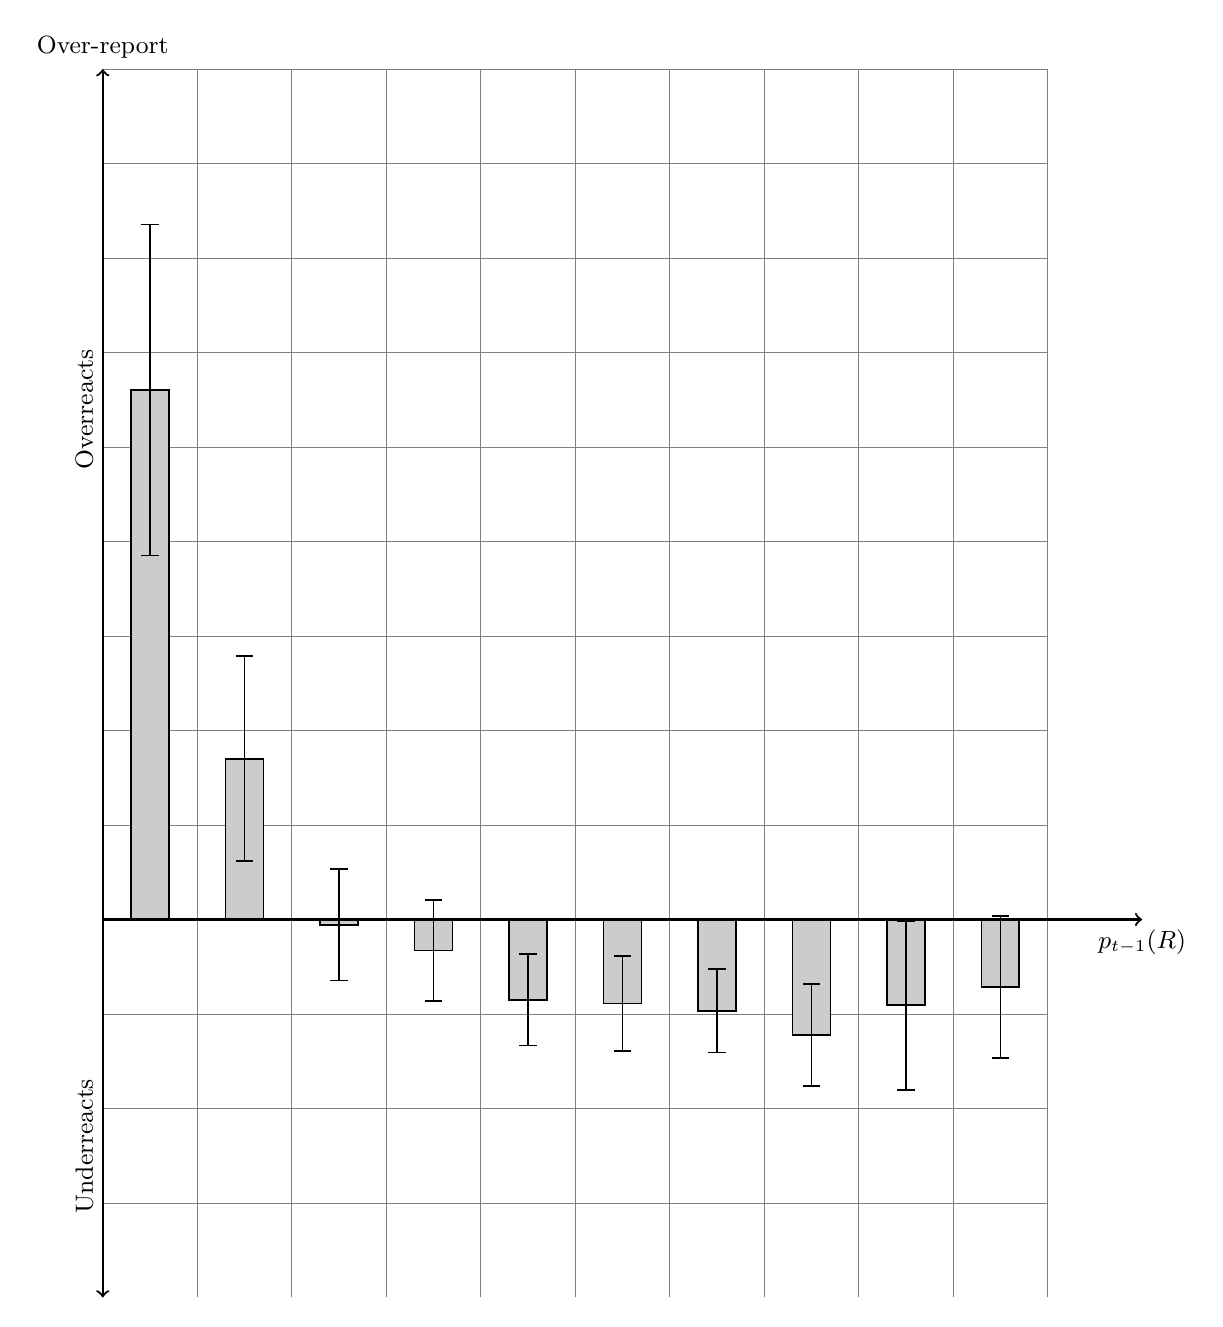
\begin{tikzpicture}[scale=12]
\draw[help lines,step=0.1] (0,-0.4) grid (1,0.9);
\filldraw[opaque,white!80!black] (0.03,0) rectangle (0.07,0.5604);
\draw[line width=0.6] (0.03,0) rectangle (0.07,0.5604);
\draw[line width=0.6,|-|] (0.05,0.3844) -- (0.05,0.7365);
\filldraw[opaque,white!80!black] (0.13,0) rectangle (0.17,0.1701);
\draw[line width=0.6] (0.13,0) rectangle (0.17,0.1701);
\draw[line width=0.6,|-|] (0.15,0.0608) -- (0.15,0.2794);
\filldraw[opaque,white!80!black] (0.23,0) rectangle (0.27,-0.0056);
\draw[line width=0.6] (0.23,0) rectangle (0.27,-0.0056);
\draw[line width=0.6,|-|] (0.25,-0.0655) -- (0.25,0.0544);
\filldraw[opaque,white!80!black] (0.33,0) rectangle (0.37,-0.0329);
\draw[line width=0.6] (0.33,0) rectangle (0.37,-0.0329);
\draw[line width=0.6,|-|] (0.35,-0.0871) -- (0.35,0.0213);
\filldraw[opaque,white!80!black] (0.43,0) rectangle (0.47,-0.0850);
\draw[line width=0.6] (0.43,0) rectangle (0.47,-0.0850);
\draw[line width=0.6,|-|] (0.45,-0.1344) -- (0.45,-0.0355);
\filldraw[opaque,white!80!black] (0.53,0) rectangle (0.57,-0.0891);
\draw[line width=0.6] (0.53,0) rectangle (0.57,-0.0891);
\draw[line width=0.6,|-|] (0.55,-0.1403) -- (0.55,-0.0379);
\filldraw[opaque,white!80!black] (0.63,0) rectangle (0.67,-0.0966);
\draw[line width=0.6] (0.63,0) rectangle (0.67,-0.0966);
\draw[line width=0.6,|-|] (0.65,-0.1415) -- (0.65,-0.0516);
\filldraw[opaque,white!80!black] (0.73,0) rectangle (0.77,-0.1223);
\draw[line width=0.6] (0.73,0) rectangle (0.77,-0.1223);
\draw[line width=0.6,|-|] (0.75,-0.1774) -- (0.75,-0.0673);
\filldraw[opaque,white!80!black] (0.83,0) rectangle (0.87,-0.0908);
\draw[line width=0.6] (0.83,0) rectangle (0.87,-0.0908);
\draw[line width=0.6,|-|] (0.85,-0.1811) -- (0.85,-0.0005);
\filldraw[opaque,white!80!black] (0.93,0) rectangle (0.97,-0.0715);
\draw[line width=0.6] (0.93,0) rectangle (0.97,-0.0715);
\draw[line width=0.6,|-|] (0.95,-0.1477) -- (0.95,0.0047);
\draw[line width=0.8,->]  (0,0) -- (1.1,0) node[below] {\small{$p_{t-1}(R)$}};
\draw[line width=0.8,<->] (0,-0.4) -- (0,0.9) node[above] {\small{Over-report}};
\draw (0,0.54) node[above,rotate=90] {\small{Overreacts}};
\draw (0,-0.24) node[above,rotate=90] {\small{Underreacts}};
% ADD THEORY CURVE BELOW
\end{tikzpicture}
}
\subcaption{$(H_{0,0})$: 0 retractions / 0 confirmations}
\end{subfigure}
\hfill
\begin{subfigure}[t]{0.485\textwidth}
\centering
\resizebox{\linewidth}{!}{
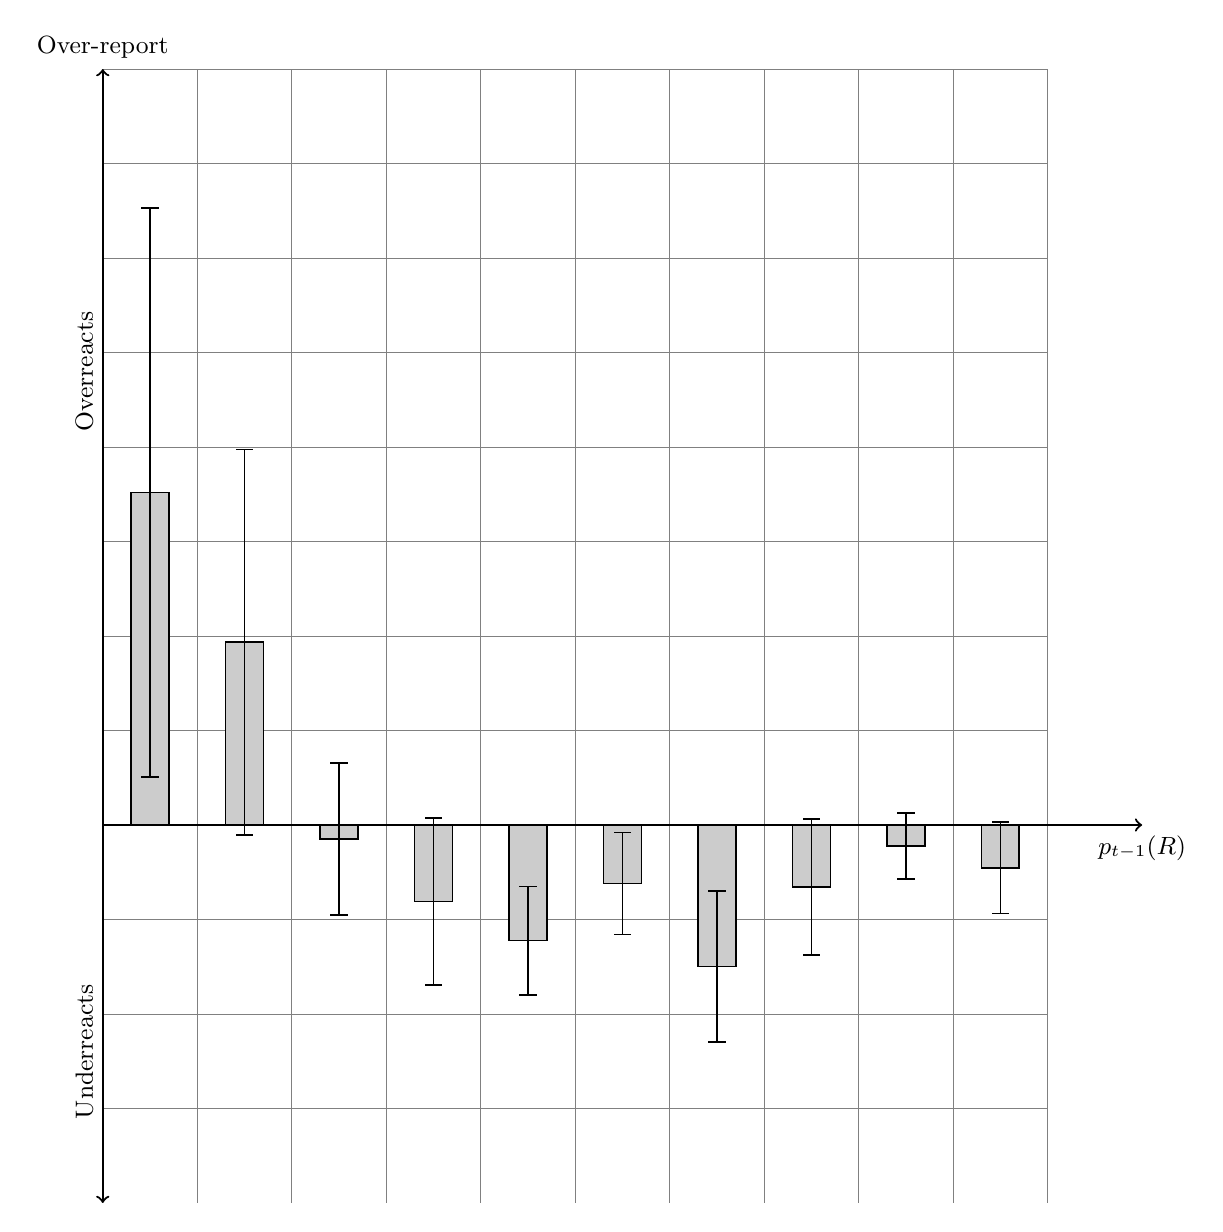
\begin{tikzpicture}[scale=12]
\draw[help lines,step=0.1] (0,-0.4) grid (1,0.8);
\filldraw[opaque,white!80!black] (0.03,0) rectangle (0.07,0.3519);
\draw[line width=0.6] (0.03,0) rectangle (0.07,0.3519);
\draw[line width=0.6,|-|] (0.05,0.0501) -- (0.05,0.6538);
\filldraw[opaque,white!80!black] (0.13,0) rectangle (0.17,0.1935);
\draw[line width=0.6] (0.13,0) rectangle (0.17,0.1935);
\draw[line width=0.6,|-|] (0.15,-0.0114) -- (0.15,0.3983);
\filldraw[opaque,white!80!black] (0.23,0) rectangle (0.27,-0.0149);
\draw[line width=0.6] (0.23,0) rectangle (0.27,-0.0149);
\draw[line width=0.6,|-|] (0.25,-0.0963) -- (0.25,0.0665);
\filldraw[opaque,white!80!black] (0.33,0) rectangle (0.37,-0.0809);
\draw[line width=0.6] (0.33,0) rectangle (0.37,-0.0809);
\draw[line width=0.6,|-|] (0.35,-0.1699) -- (0.35,0.0082);
\filldraw[opaque,white!80!black] (0.43,0) rectangle (0.47,-0.1224);
\draw[line width=0.6] (0.43,0) rectangle (0.47,-0.1224);
\draw[line width=0.6,|-|] (0.45,-0.1806) -- (0.45,-0.0642);
\filldraw[opaque,white!80!black] (0.53,0) rectangle (0.57,-0.0619);
\draw[line width=0.6] (0.53,0) rectangle (0.57,-0.0619);
\draw[line width=0.6,|-|] (0.55,-0.1166) -- (0.55,-0.0071);
\filldraw[opaque,white!80!black] (0.63,0) rectangle (0.67,-0.1496);
\draw[line width=0.6] (0.63,0) rectangle (0.67,-0.1496);
\draw[line width=0.6,|-|] (0.65,-0.2304) -- (0.65,-0.0689);
\filldraw[opaque,white!80!black] (0.73,0) rectangle (0.77,-0.0657);
\draw[line width=0.6] (0.73,0) rectangle (0.77,-0.0657);
\draw[line width=0.6,|-|] (0.75,-0.1384) -- (0.75,0.0070);
\filldraw[opaque,white!80!black] (0.83,0) rectangle (0.87,-0.0224);
\draw[line width=0.6] (0.83,0) rectangle (0.87,-0.0224);
\draw[line width=0.6,|-|] (0.85,-0.0580) -- (0.85,0.0133);
\filldraw[opaque,white!80!black] (0.93,0) rectangle (0.97,-0.0453);
\draw[line width=0.6] (0.93,0) rectangle (0.97,-0.0453);
\draw[line width=0.6,|-|] (0.95,-0.0944) -- (0.95,0.0038);
\draw[line width=0.8,->]  (0,0) -- (1.1,0) node[below] {\small{$p_{t-1}(R)$}};
\draw[line width=0.8,<->] (0,-0.4) -- (0,0.8) node[above] {\small{Over-report}};
\draw (0,0.48) node[above,rotate=90] {\small{Overreacts}};
\draw (0,-0.24) node[above,rotate=90] {\small{Underreacts}};
% ADD THEORY CURVE BELOW
\end{tikzpicture}
}
\subcaption{$(H_{1,0})$: 1 retraction / 0 confirmations}
\end{subfigure}
\\[1.5ex]
\begin{subfigure}[t]{0.485\textwidth}
\centering
\resizebox{\linewidth}{!}{
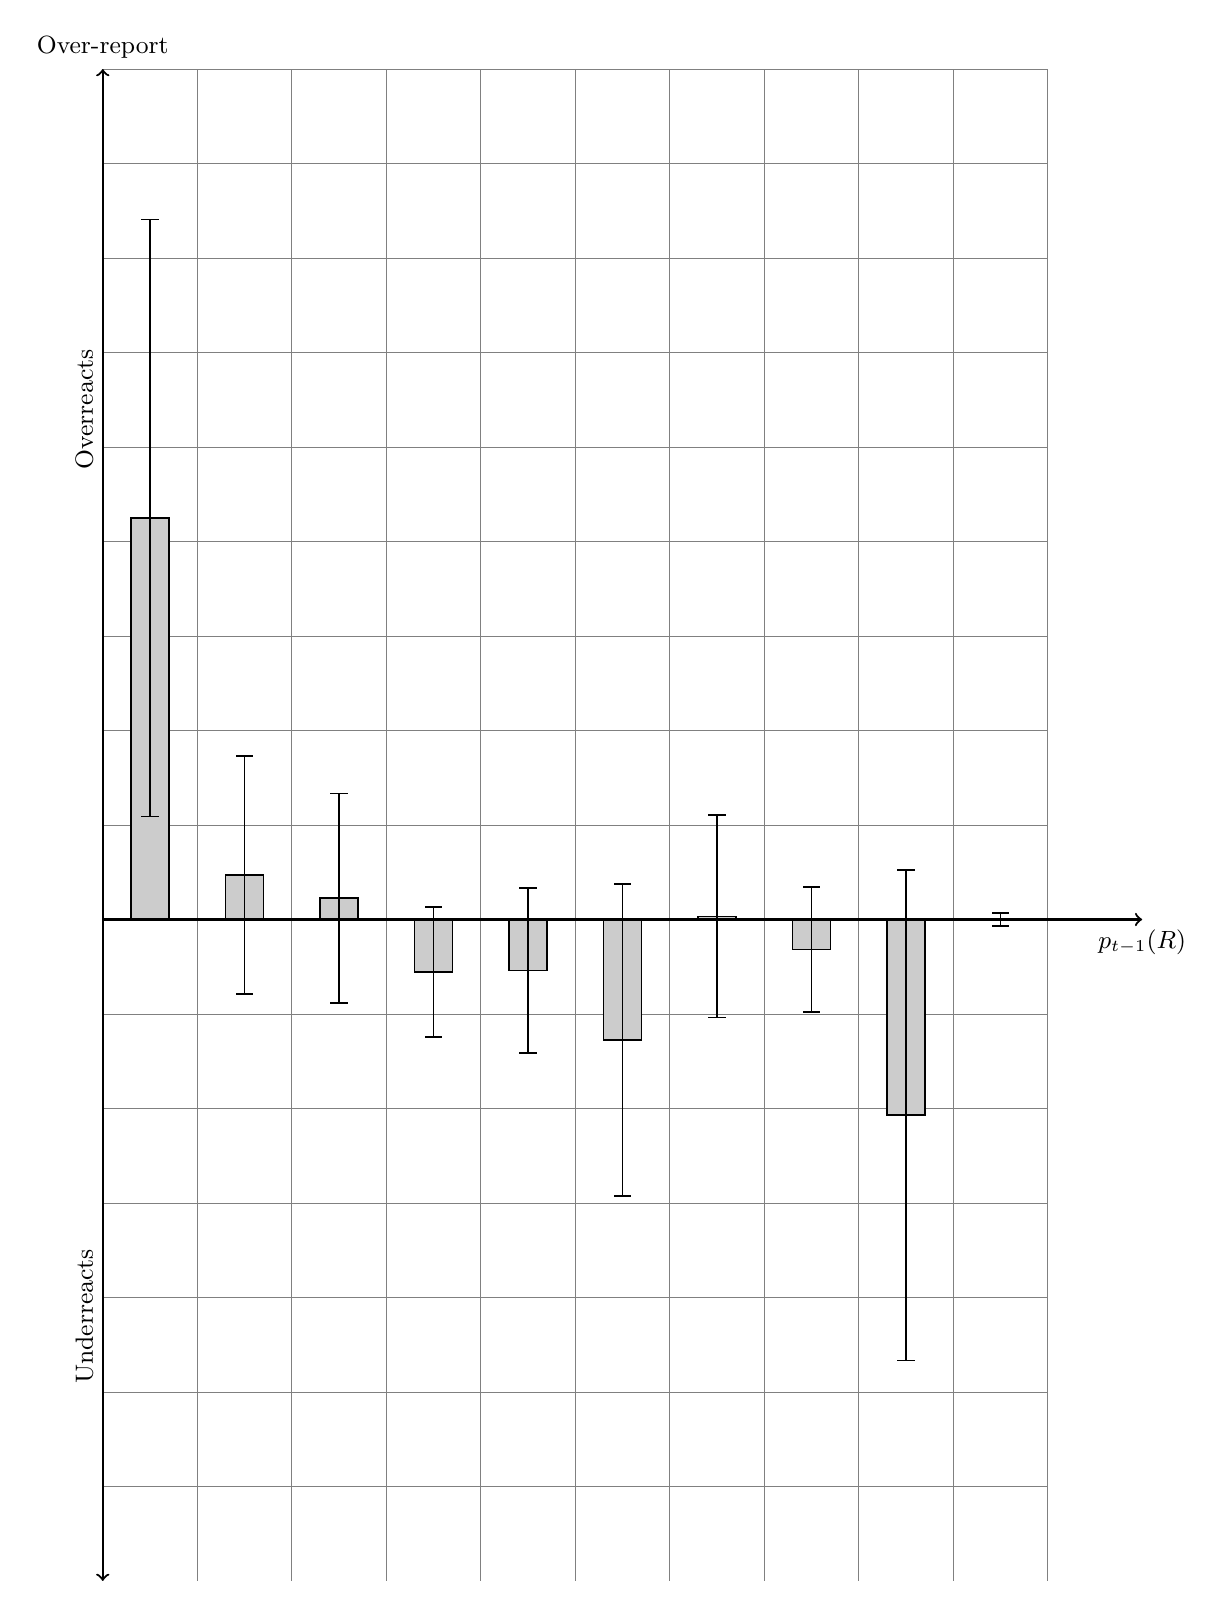
\begin{tikzpicture}[scale=12]
\draw[help lines,step=0.1] (0,-0.7) grid (1,0.9);
\filldraw[opaque,white!80!black] (0.03,0) rectangle (0.07,0.4250);
\draw[line width=0.6] (0.03,0) rectangle (0.07,0.4250);
\draw[line width=0.6,|-|] (0.05,0.1082) -- (0.05,0.7418);
\filldraw[opaque,white!80!black] (0.13,0) rectangle (0.17,0.0472);
\draw[line width=0.6] (0.13,0) rectangle (0.17,0.0472);
\draw[line width=0.6,|-|] (0.15,-0.0797) -- (0.15,0.1740);
\filldraw[opaque,white!80!black] (0.23,0) rectangle (0.27,0.0224);
\draw[line width=0.6] (0.23,0) rectangle (0.27,0.0224);
\draw[line width=0.6,|-|] (0.25,-0.0894) -- (0.25,0.1341);
\filldraw[opaque,white!80!black] (0.33,0) rectangle (0.37,-0.0558);
\draw[line width=0.6] (0.33,0) rectangle (0.37,-0.0558);
\draw[line width=0.6,|-|] (0.35,-0.1255) -- (0.35,0.0139);
\filldraw[opaque,white!80!black] (0.43,0) rectangle (0.47,-0.0539);
\draw[line width=0.6] (0.43,0) rectangle (0.47,-0.0539);
\draw[line width=0.6,|-|] (0.45,-0.1423) -- (0.45,0.0345);
\filldraw[opaque,white!80!black] (0.53,0) rectangle (0.57,-0.1275);
\draw[line width=0.6] (0.53,0) rectangle (0.57,-0.1275);
\draw[line width=0.6,|-|] (0.55,-0.2935) -- (0.55,0.0385);
\filldraw[opaque,white!80!black] (0.63,0) rectangle (0.67,0.0033);
\draw[line width=0.6] (0.63,0) rectangle (0.67,0.0033);
\draw[line width=0.6,|-|] (0.65,-0.1048) -- (0.65,0.1114);
\filldraw[opaque,white!80!black] (0.73,0) rectangle (0.77,-0.0317);
\draw[line width=0.6] (0.73,0) rectangle (0.77,-0.0317);
\draw[line width=0.6,|-|] (0.75,-0.0990) -- (0.75,0.0356);
\filldraw[opaque,white!80!black] (0.83,0) rectangle (0.87,-0.2072);
\draw[line width=0.6] (0.83,0) rectangle (0.87,-0.2072);
\draw[line width=0.6,|-|] (0.85,-0.4677) -- (0.85,0.0533);
\filldraw[opaque,white!80!black] (0.93,0) rectangle (0.97,-0.0001);
\draw[line width=0.6] (0.93,0) rectangle (0.97,-0.0001);
\draw[line width=0.6,|-|] (0.95,-0.0081) -- (0.95,0.0079);
\draw[line width=0.8,->]  (0,0) -- (1.1,0) node[below] {\small{$p_{t-1}(R)$}};
\draw[line width=0.8,<->] (0,-0.7) -- (0,0.9) node[above] {\small{Over-report}};
\draw (0,0.54) node[above,rotate=90] {\small{Overreacts}};
\draw (0,-0.42) node[above,rotate=90] {\small{Underreacts}};
% ADD THEORY CURVE BELOW
\end{tikzpicture}
}
\subcaption{$(H_{0,1})$: 0 retractions / 1 confirmation}
\end{subfigure}
\hfill
\begin{subfigure}[t]{0.485\textwidth}
\centering
\resizebox{\linewidth}{!}{
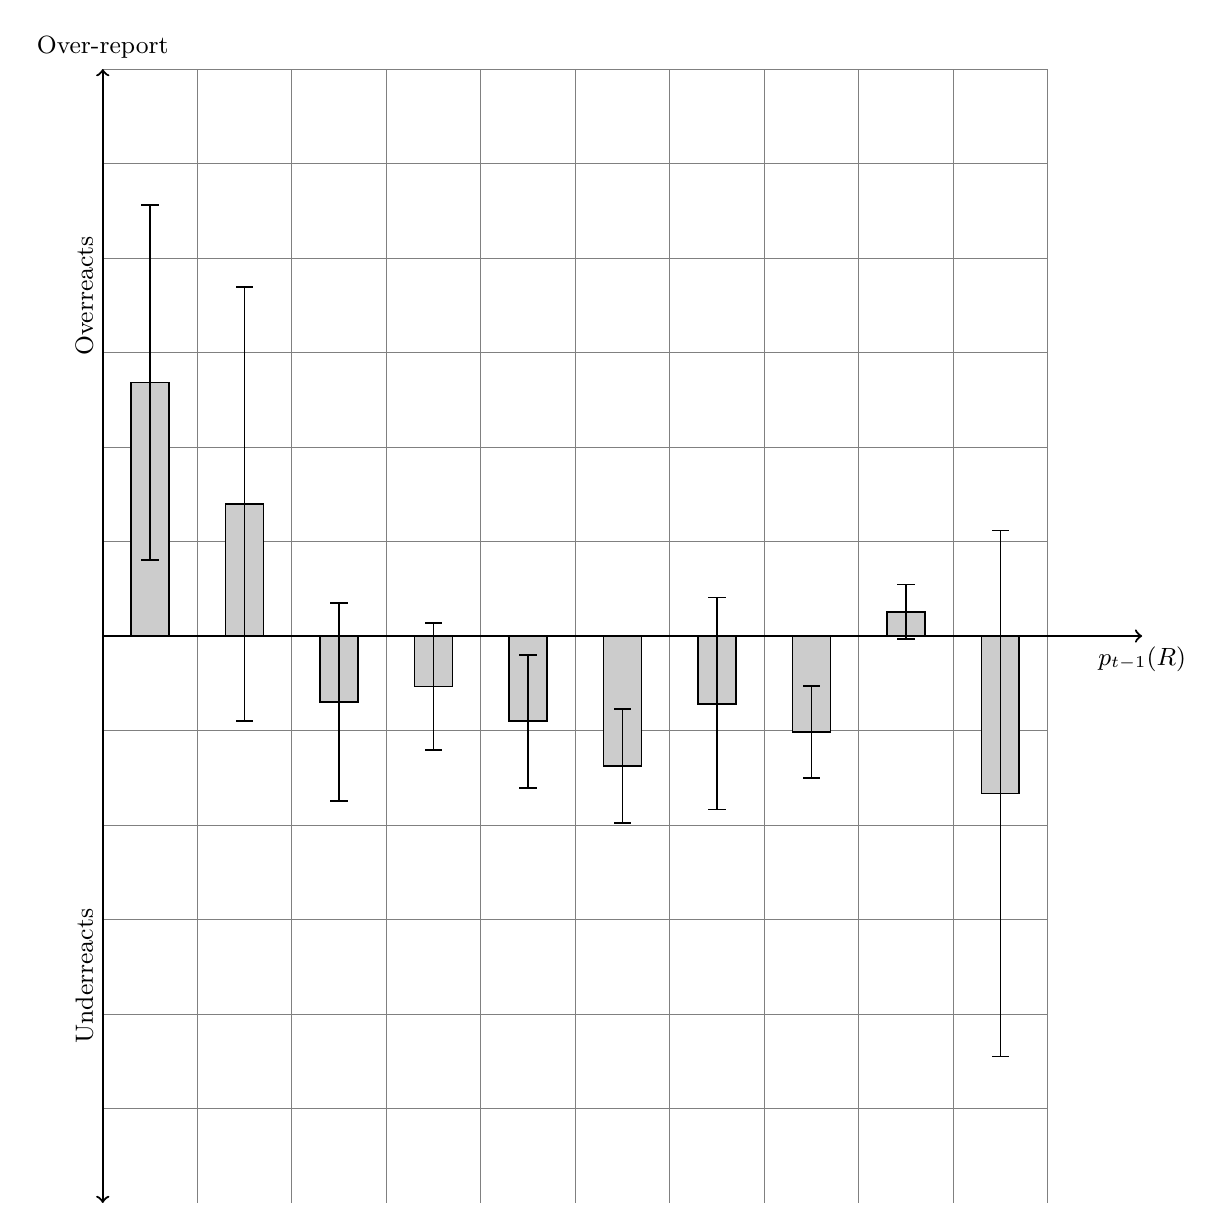
\begin{tikzpicture}[scale=12]
\draw[help lines,step=0.1] (0,-0.6) grid (1,0.6);
\filldraw[opaque,white!80!black] (0.03,0) rectangle (0.07,0.2683);
\draw[line width=0.6] (0.03,0) rectangle (0.07,0.2683);
\draw[line width=0.6,|-|] (0.05,0.0796) -- (0.05,0.4570);
\filldraw[opaque,white!80!black] (0.13,0) rectangle (0.17,0.1398);
\draw[line width=0.6] (0.13,0) rectangle (0.17,0.1398);
\draw[line width=0.6,|-|] (0.15,-0.0911) -- (0.15,0.3706);
\filldraw[opaque,white!80!black] (0.23,0) rectangle (0.27,-0.0697);
\draw[line width=0.6] (0.23,0) rectangle (0.27,-0.0697);
\draw[line width=0.6,|-|] (0.25,-0.1755) -- (0.25,0.0361);
\filldraw[opaque,white!80!black] (0.33,0) rectangle (0.37,-0.0534);
\draw[line width=0.6] (0.33,0) rectangle (0.37,-0.0534);
\draw[line width=0.6,|-|] (0.35,-0.1218) -- (0.35,0.0150);
\filldraw[opaque,white!80!black] (0.43,0) rectangle (0.47,-0.0901);
\draw[line width=0.6] (0.43,0) rectangle (0.47,-0.0901);
\draw[line width=0.6,|-|] (0.45,-0.1614) -- (0.45,-0.0189);
\filldraw[opaque,white!80!black] (0.53,0) rectangle (0.57,-0.1375);
\draw[line width=0.6] (0.53,0) rectangle (0.57,-0.1375);
\draw[line width=0.6,|-|] (0.55,-0.1989) -- (0.55,-0.0761);
\filldraw[opaque,white!80!black] (0.63,0) rectangle (0.67,-0.0716);
\draw[line width=0.6] (0.63,0) rectangle (0.67,-0.0716);
\draw[line width=0.6,|-|] (0.65,-0.1846) -- (0.65,0.0415);
\filldraw[opaque,white!80!black] (0.73,0) rectangle (0.77,-0.1015);
\draw[line width=0.6] (0.73,0) rectangle (0.77,-0.1015);
\draw[line width=0.6,|-|] (0.75,-0.1508) -- (0.75,-0.0523);
\filldraw[opaque,white!80!black] (0.83,0) rectangle (0.87,0.0256);
\draw[line width=0.6] (0.83,0) rectangle (0.87,0.0256);
\draw[line width=0.6,|-|] (0.85,-0.0043) -- (0.85,0.0555);
\filldraw[opaque,white!80!black] (0.93,0) rectangle (0.97,-0.1667);
\draw[line width=0.6] (0.93,0) rectangle (0.97,-0.1667);
\draw[line width=0.6,|-|] (0.95,-0.4458) -- (0.95,0.1124);
\draw[line width=0.8,->]  (0,0) -- (1.1,0) node[below] {\small{$p_{t-1}(R)$}};
\draw[line width=0.8,<->] (0,-0.6) -- (0,0.6) node[above] {\small{Over-report}};
\draw (0,0.36) node[above,rotate=90] {\small{Overreacts}};
\draw (0,-0.36) node[above,rotate=90] {\small{Underreacts}};
% ADD THEORY CURVE BELOW
\end{tikzpicture}
}
\subcaption{$(H_{2,0})$: 2 retractions / 0 confirmations}
\end{subfigure}
\\[1.5ex]
\begin{subfigure}[t]{0.485\textwidth}
\centering
\resizebox{\linewidth}{!}{
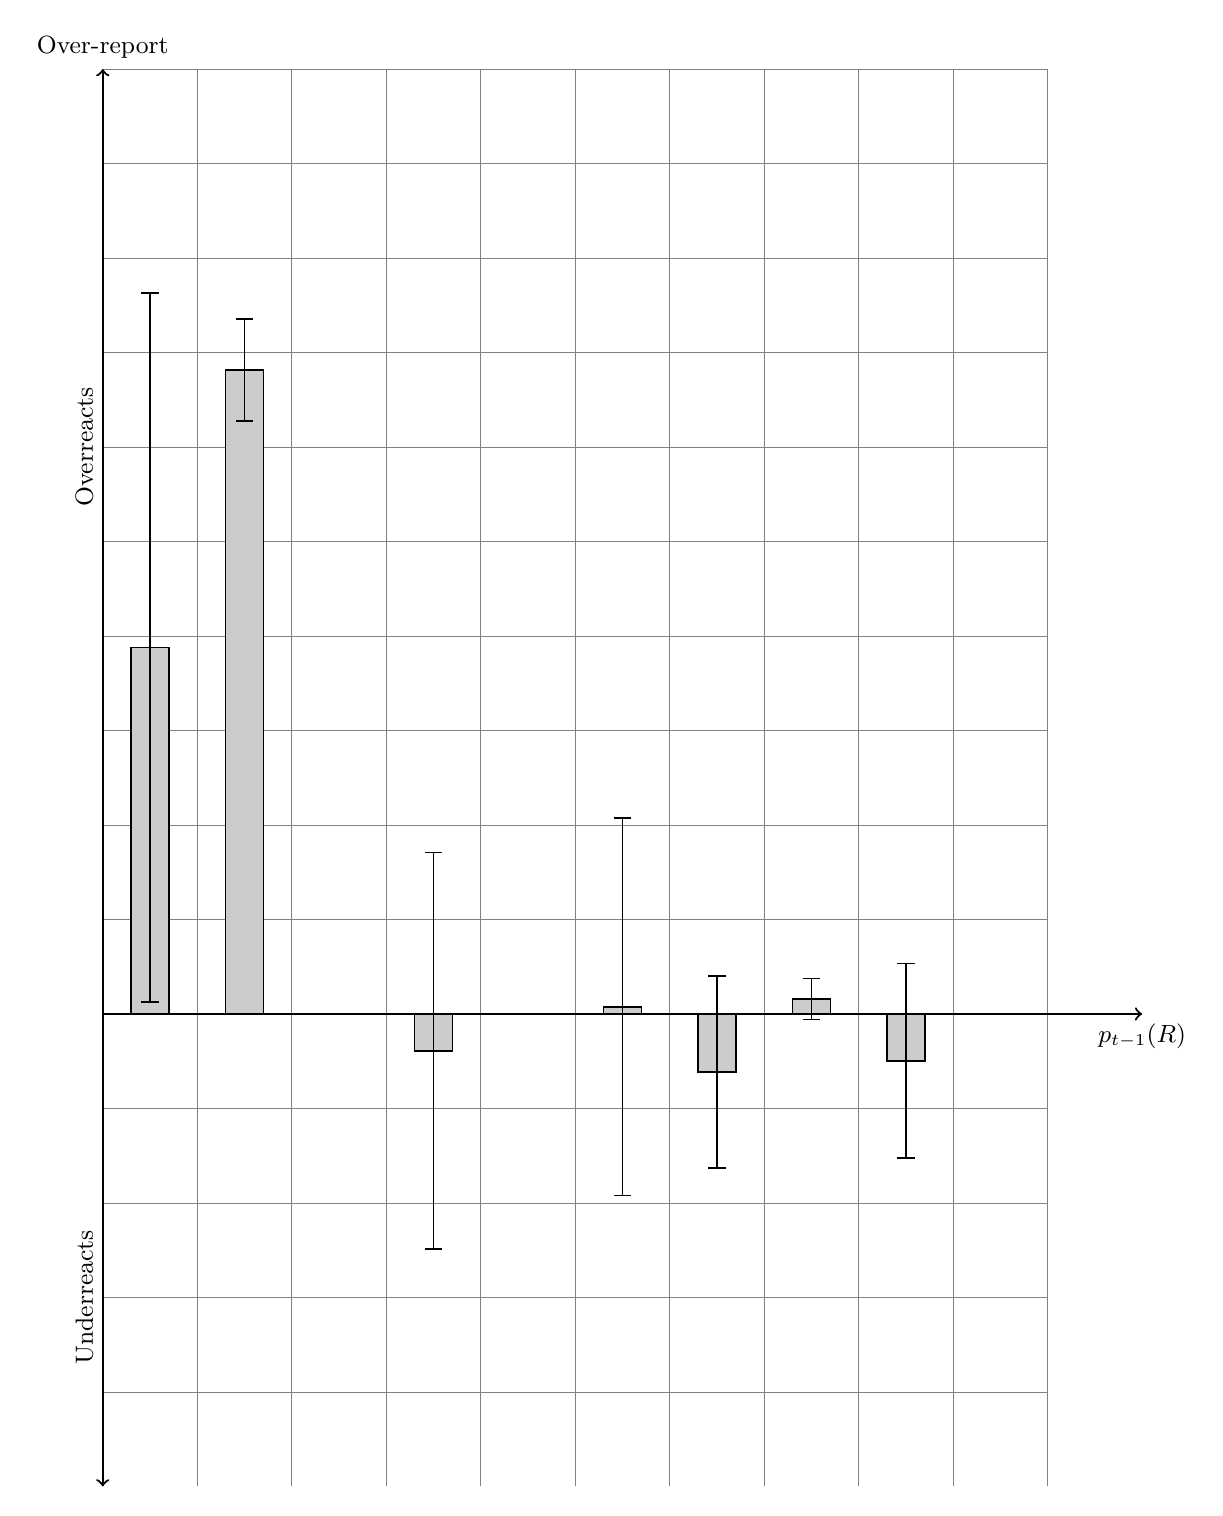
\begin{tikzpicture}[scale=12]
\draw[help lines,step=0.1] (0,-0.5) grid (1,1.0);
\filldraw[opaque,white!80!black] (0.03,0) rectangle (0.07,0.3879);
\draw[line width=0.6] (0.03,0) rectangle (0.07,0.3879);
\draw[line width=0.6,|-|] (0.05,0.0118) -- (0.05,0.7640);
\filldraw[opaque,white!80!black] (0.13,0) rectangle (0.17,0.6818);
\draw[line width=0.6] (0.13,0) rectangle (0.17,0.6818);
\draw[line width=0.6,|-|] (0.15,0.6270) -- (0.15,0.7365);
\filldraw[opaque,white!80!black] (0.33,0) rectangle (0.37,-0.0391);
\draw[line width=0.6] (0.33,0) rectangle (0.37,-0.0391);
\draw[line width=0.6,|-|] (0.35,-0.2499) -- (0.35,0.1717);
\filldraw[opaque,white!80!black] (0.53,0) rectangle (0.57,0.0077);
\draw[line width=0.6] (0.53,0) rectangle (0.57,0.0077);
\draw[line width=0.6,|-|] (0.55,-0.1931) -- (0.55,0.2085);
\filldraw[opaque,white!80!black] (0.63,0) rectangle (0.67,-0.0614);
\draw[line width=0.6] (0.63,0) rectangle (0.67,-0.0614);
\draw[line width=0.6,|-|] (0.65,-0.1637) -- (0.65,0.0410);
\filldraw[opaque,white!80!black] (0.73,0) rectangle (0.77,0.0157);
\draw[line width=0.6] (0.73,0) rectangle (0.77,0.0157);
\draw[line width=0.6,|-|] (0.75,-0.0069) -- (0.75,0.0383);
\filldraw[opaque,white!80!black] (0.83,0) rectangle (0.87,-0.0495);
\draw[line width=0.6] (0.83,0) rectangle (0.87,-0.0495);
\draw[line width=0.6,|-|] (0.85,-0.1532) -- (0.85,0.0543);
\draw[line width=0.8,->]  (0,0) -- (1.1,0) node[below] {\small{$p_{t-1}(R)$}};
\draw[line width=0.8,<->] (0,-0.5) -- (0,1.0) node[above] {\small{Over-report}};
\draw (0,0.60) node[above,rotate=90] {\small{Overreacts}};
\draw (0,-0.30) node[above,rotate=90] {\small{Underreacts}};
% ADD THEORY CURVE BELOW
\end{tikzpicture}
}
\subcaption{$(H_{0,2})$: 0 retractions / 2 confirmations}
\end{subfigure}
\hfill
\begin{subfigure}[t]{0.485\textwidth}
\centering
\resizebox{\linewidth}{!}{
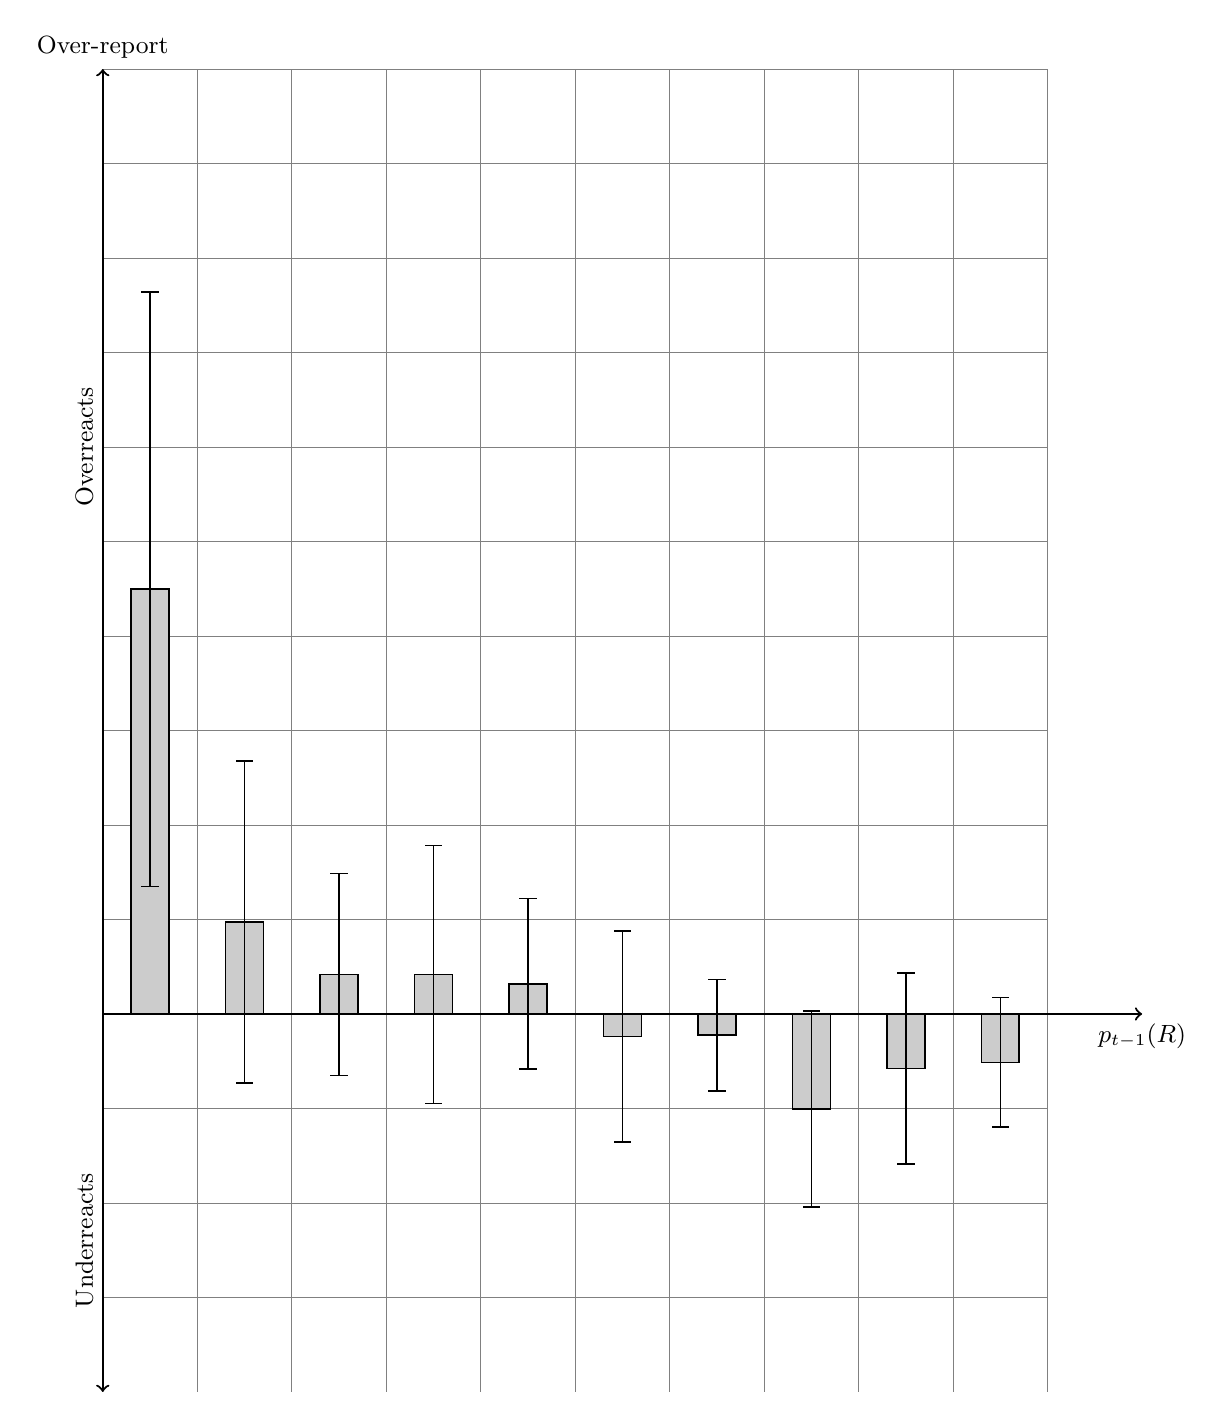
\begin{tikzpicture}[scale=12]
\draw[help lines,step=0.1] (0,-0.4) grid (1,1.0);
\filldraw[opaque,white!80!black] (0.03,0) rectangle (0.07,0.4496);
\draw[line width=0.6] (0.03,0) rectangle (0.07,0.4496);
\draw[line width=0.6,|-|] (0.05,0.1341) -- (0.05,0.7652);
\filldraw[opaque,white!80!black] (0.13,0) rectangle (0.17,0.0971);
\draw[line width=0.6] (0.13,0) rectangle (0.17,0.0971);
\draw[line width=0.6,|-|] (0.15,-0.0742) -- (0.15,0.2684);
\filldraw[opaque,white!80!black] (0.23,0) rectangle (0.27,0.0417);
\draw[line width=0.6] (0.23,0) rectangle (0.27,0.0417);
\draw[line width=0.6,|-|] (0.25,-0.0659) -- (0.25,0.1494);
\filldraw[opaque,white!80!black] (0.33,0) rectangle (0.37,0.0418);
\draw[line width=0.6] (0.33,0) rectangle (0.37,0.0418);
\draw[line width=0.6,|-|] (0.35,-0.0956) -- (0.35,0.1792);
\filldraw[opaque,white!80!black] (0.43,0) rectangle (0.47,0.0320);
\draw[line width=0.6] (0.43,0) rectangle (0.47,0.0320);
\draw[line width=0.6,|-|] (0.45,-0.0591) -- (0.45,0.1230);
\filldraw[opaque,white!80!black] (0.53,0) rectangle (0.57,-0.0239);
\draw[line width=0.6] (0.53,0) rectangle (0.57,-0.0239);
\draw[line width=0.6,|-|] (0.55,-0.1365) -- (0.55,0.0887);
\filldraw[opaque,white!80!black] (0.63,0) rectangle (0.67,-0.0223);
\draw[line width=0.6] (0.63,0) rectangle (0.67,-0.0223);
\draw[line width=0.6,|-|] (0.65,-0.0821) -- (0.65,0.0375);
\filldraw[opaque,white!80!black] (0.73,0) rectangle (0.77,-0.1004);
\draw[line width=0.6] (0.73,0) rectangle (0.77,-0.1004);
\draw[line width=0.6,|-|] (0.75,-0.2049) -- (0.75,0.0042);
\filldraw[opaque,white!80!black] (0.83,0) rectangle (0.87,-0.0577);
\draw[line width=0.6] (0.83,0) rectangle (0.87,-0.0577);
\draw[line width=0.6,|-|] (0.85,-0.1596) -- (0.85,0.0442);
\filldraw[opaque,white!80!black] (0.93,0) rectangle (0.97,-0.0512);
\draw[line width=0.6] (0.93,0) rectangle (0.97,-0.0512);
\draw[line width=0.6,|-|] (0.95,-0.1208) -- (0.95,0.0184);
\draw[line width=0.8,->]  (0,0) -- (1.1,0) node[below] {\small{$p_{t-1}(R)$}};
\draw[line width=0.8,<->] (0,-0.4) -- (0,1.0) node[above] {\small{Over-report}};
\draw (0,0.60) node[above,rotate=90] {\small{Overreacts}};
\draw (0,-0.24) node[above,rotate=90] {\small{Underreacts}};
% ADD THEORY CURVE BELOW
\end{tikzpicture}
}
\subcaption{$(H_{1,1})$: 1 retraction / 1 confirmation}
\end{subfigure}
